%%%%%%%%%%%%%%%%%%%%%%%%%%%%%%%%%%%%%%%%%
% Short Sectioned Assignment
% LaTeX Template
% Version 1.0 (5/5/12)
%
% This template has been downloaded from:
% http://www.LaTeXTemplates.com
%
% Original author:
% Frits Wenneker (http://www.howtotex.com)
%
% License:
% CC BY-NC-SA 3.0 (http://creativecommons.org/licenses/by-nc-sa/3.0/)
%
%%%%%%%%%%%%%%%%%%%%%%%%%%%%%%%%%%%%%%%%%

%----------------------------------------------------------------------------------------
%	PACKAGES AND OTHER DOCUMENT CONFIGURATIONS
%----------------------------------------------------------------------------------------

\documentclass[paper=a4, fontsize=11pt]{scrartcl} % A4 paper and 11pt font size

\usepackage[T1]{fontenc} % Use 8-bit encoding that has 256 glyphs
\usepackage{fourier} % Use the Adobe Utopia font for the document - comment this line to return to the LaTeX default
\usepackage[english]{babel} % English language/hyphenation
\usepackage{amsmath,amsfonts,amsthm} % Math packages

\usepackage{graphicx}

\usepackage{sectsty} % Allows customizing section commands
\allsectionsfont{\centering \normalfont\scshape} % Make all sections centered, the default font and small caps

\usepackage{fancyhdr} % Custom headers and footers
\pagestyle{fancyplain} % Makes all pages in the document conform to the custom headers and footers
\fancyhead{} % No page header - if you want one, create it in the same way as the footers below
\fancyfoot[L]{} % Empty left footer
\fancyfoot[C]{} % Empty center footer
\fancyfoot[R]{\thepage} % Page numbering for right footer
\renewcommand{\headrulewidth}{0pt} % Remove header underlines
\renewcommand{\footrulewidth}{0pt} % Remove footer underlines
\setlength{\headheight}{13.6pt} % Customize the height of the header

\numberwithin{equation}{section} % Number equations within sections (i.e. 1.1, 1.2, 2.1, 2.2 instead of 1, 2, 3, 4)
\numberwithin{figure}{section} % Number figures within sections (i.e. 1.1, 1.2, 2.1, 2.2 instead of 1, 2, 3, 4)
\numberwithin{table}{section} % Number tables within sections (i.e. 1.1, 1.2, 2.1, 2.2 instead of 1, 2, 3, 4)

\setlength\parindent{0pt} % Removes all indentation from paragraphs - comment this line for an assignment with lots of text

%----------------------------------------------------------------------------------------
%	TITLE SECTION
%----------------------------------------------------------------------------------------

\newcommand{\horrule}[1]{\rule{\linewidth}{#1}} % Create horizontal rule command with 1 argument of height

\title{	
\normalfont \normalsize 
\textsc{BRSU} \\ [25pt] % Your university, school and/or department name(s)
\horrule{0.5pt} \\[0.4cm] % Thin top horizontal rule
\huge Homework for Artificial Intelligence for Robotics - Assignment 4 \\ % The assignment title
\horrule{2pt} \\[0.5cm] % Thick bottom horizontal rule
}

\author{Bastian Lang} % Your name

\date{\normalsize\today} % Today's date or a custom date

\begin{document}

\maketitle % Print the title

\section{Theoretical Part}
\subsection{Exercise 1}
\emph{Describe an example state space or problem in which iterative deepening search performs
much worse than depth-first search.}\\\\

Iterative deepening search has a space complexity equal to depth first search, so the difference has to be in the time complexity.\\
Iterative deepening search is able to find solutions in relatively small depth without having to first entirely search other parts of the tree.\\
On the other hand equal to breadth first search it first completely expands each level before proceeding to the next level.\\
A state space where depth first search would perform much better than iterative deepening search would have to have its solution at a very deep level in the search tree and it has to have a high branching factor.\\
A possible problem could be for an agent located in a cube has to reach the edge of the cube. Its actions would be to move up, down, back, forth, left or right.\\
DFS would go in a straight line until it reaches one edge. Iterative deepening search would search in expanding circles around the start location, resulting in a very high time complexity if the starting position is not directly at an edge.



\section{Practical Part}
\subsection{Task Overview}
For the practical part of this assignment we were given three ASCII maps containing obstacles, a start position and some numbered target positions.\\
The task was to implement iterative deepening depth first search to have an agent starting at the start position find a path to all the different goals, starting from the one with the lowest number.\\
The last target should be the start for the path to the next target. The agent is allowed to move up, down, left or right and it cannot move through obstacles.\\

\subsection{Approach}
Iterative deepening depth first search basically uses depth first search, but it uses a limit for the maximum depth it searches the search tree. This depth limit starts with zero and is increased by one in each incrementation. This leads to a strategy that searches the search tree in a breadth first order, but has the space complexity of depth first search.\\\\

Besides some of the helper classes and methods from the previous assignment I divided my application into the following parts. 

\subsubsection{Finding a path from start to target}
This part is focused solely on finding a path from a given position to a given target element. It results in a sequence of positions or in an empty list if there is no valid path to the given target.\\
To prune the search tree and reduce the time complexity I used a List to store the visited nodes so far.\\
I use a modified version of the depth first search algorithm. This time I have an extra loop around the algorithm increasing the depth limit as long as the algorithm had to abort because of the depth limit.\\
The difference now is that a node only gets expanded if the depth limit is not reached yet.

\subsubsection{Find a path from the start position to all targets in ascending order}
To find a path from a given position to all targets in the map in ascending order I first have to identify all the targets in the map. I just scan the map for any integer, put them in a list and have it ordered.\\
Then I call the algorithm to find a path from a start position to a given element for every target. Each time I attach the result to the path the agent found so far. For every iteration the last position in the path works as the new starting position. Therefore even if there is a target that is not reachable, the agent just tries to find a path from the last found target to the next target.

\subsubsection{Visualization}
To display the path in the map I created a JFrame that displays the map and the path that has been found.

\subsection{Results}
The results can be seen in the figures of this section. In the beginning I would have this approach to always find the optimal and shortest paths to the targets. But keeping track of the nodes visited and also of those already stored for further expansion also prunes optimal solutions.\\
After removing checks on those lists when adding new nodes to the expansion list the runtime went up so high that is was not possible to compute paths. Therefore I decided to keep those checks, what resulted in these suboptimal paths. For optimal paths one would have to skip those checks and add a maximum depth limit. But this would increase the computation time drastically.

\subsubsection{Map 1}
\begin{figure}[Ht]
	\centering
  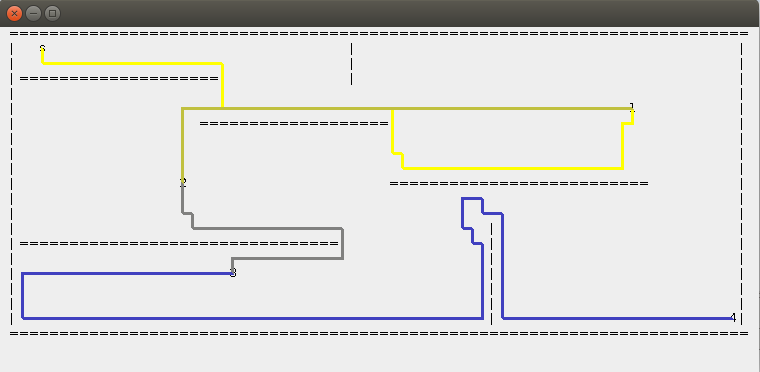
\includegraphics[width=1\textwidth]{images/map1.png}
	\caption{Path for map1}
	\label{fig:map1}
\end{figure}
\textbf{Maximum number of nodes stored in expansion list:} 137\\
\textbf{Overall nodes visited:} 70850\\
See figure \ref{fig:map1}.

\subsubsection{Map 2}
\begin{figure}[Ht]
	\centering
  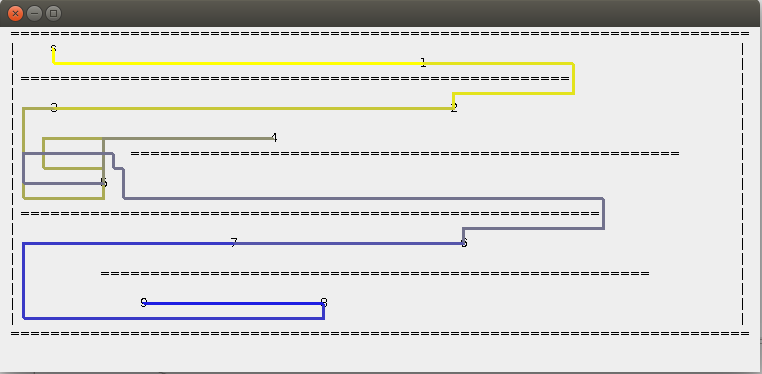
\includegraphics[width=1\textwidth]{images/map2.png}
	\caption{Path for map2}
	\label{fig:map2}
\end{figure}
\textbf{Maximum number of nodes stored in expansion list:} 96\\
\textbf{Overall nodes visited:} 52857\\
See figure \ref{fig:map2}.

\subsubsection{Map 3}
Map 3 is special because one goal is not reachable. Therefore the algorithm explores the whole map at this point before skipping this goal.\\

\begin{figure}[Ht]
	\centering
  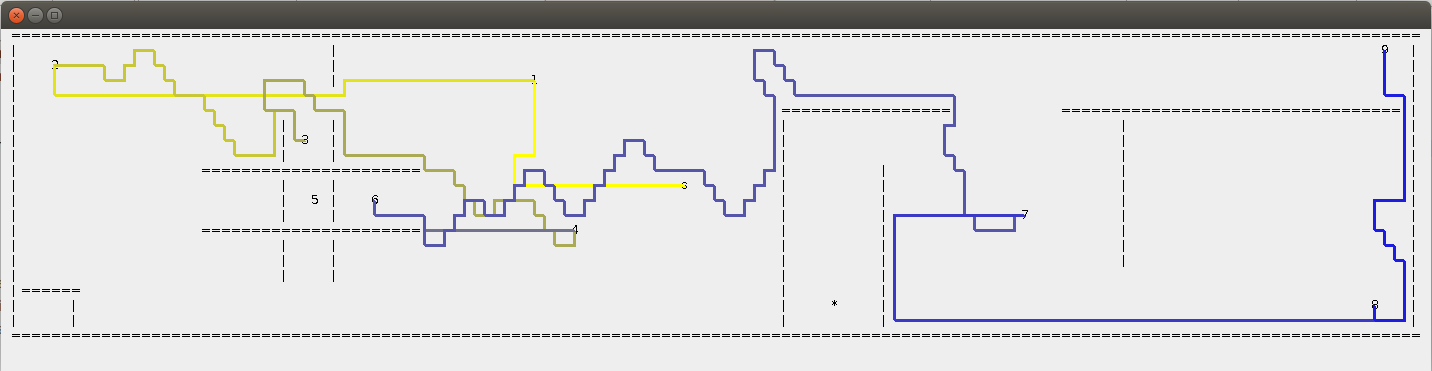
\includegraphics[width=1\textwidth]{images/map3.png}
	\caption{Path for map3}
	\label{fig:map3}
\end{figure}
\textbf{Maximum number of nodes stored in expansion list:} 864\\
\textbf{Overall nodes visited:} 1963943\\
See figure \ref{fig:map3}.\\


\end{document}